
\chapter{Steady-State Geometry Modelling}\label{ch:modelling} 

Explain the need for a model. talk about pre fabrication parameter tuning. Talk about steady state vs dynamic modelling. Explain what is told in this chapter.

\blindtext[1]

\section{Experiment Process}

Talk about the deposition of material in lines. 

Talk about the fact that first all lines are deposited. Afterwards teh measurement takes place at constant speed. Therefore having a constant sampling time and therefore equal space between measurements. Since the sampling time is unkonwn the output is scaled in time to match 
Talk about the experiment. 

Add photos of the experiment.

Add table of input parameters. 

Talk about what is being measured.

\begin{figure}[ht]
\centering
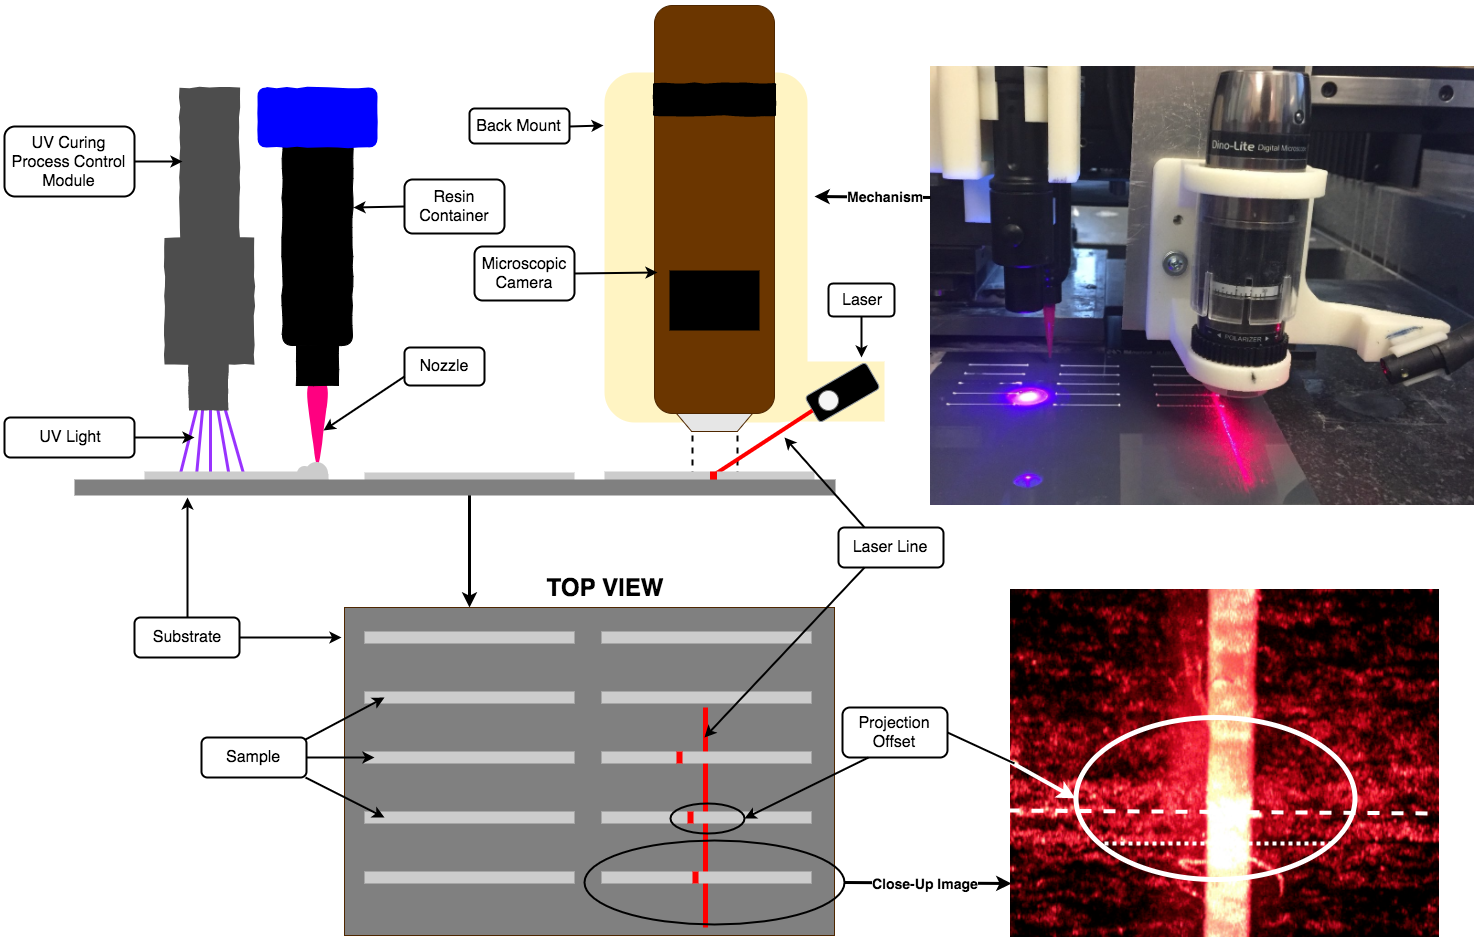
\includegraphics[width=1\linewidth]{VisionSystem} 
\caption{Experimental setup.}
\label{fig: setup}
\end{figure}

\blindtext[3]

\section{Data Cleaning}

Talk about extracting the steady state part of the detection. Talk about artifacts in the measurements to clear differences in the experiment execution.

\blindtext[6]

\section{Data Based Modelling}

The generated models. 

Make visuals of the models

\blindtext[8]